%\documentclass[12pt,draftcls,onecolumn]{IEEEtran}
%\documentclass[12pt,twocolumn]{IEEEtran}
\documentclass[twocolumn]{IEEEtran}
\usepackage{times}
%!TEX root =  autocontgrlp.tex
\usepackage{etex}
\usepackage{multicol}
\setlength{\marginparwidth}{13mm}
\usepackage[textsize=tiny]{todonotes}
%\usepackage[disable]{todonotes}
\newcommand{\todoc}[2][]{\todo[color=red!20!white,#1]{Cs: #2}}
\newcommand{\todoch}[2][]{\todo[color=blue!20!white,#1]{C: #2}}
\newcommand{\todos}[2][]{\todo[inline,color=blue!20!white,#1]{S: #2}}
%\usepackage{enumitem}
%\usepackage[fleqn]{amsmath}
\usepackage{amsmath}
\usepackage{mathtools}
\usepackage{graphicx}
\usepackage{times}
\usepackage{helvet}
\usepackage{courier}
\usepackage{paralist}
\usepackage{latexsym}
\usepackage{url}
\usepackage[all]{xy}
\usepackage{amsmath}
\usepackage{amssymb}
\usepackage{amsthm}
\usepackage{nccmath} % mfrac
\usepackage{comment}
%\usepackage{enumitem}
\usepackage{paralist}
\usepackage{xcolor}
\usepackage[colorlinks=true,linkcolor=blue,citecolor=purple]{hyperref}
%\usepackage{hyperref}
\usepackage{graphicx}
\usepackage{pifont}
%\usepackage{algorithm}
%\usepackage{algorithmic}
%\usepackage{pseudocode}
%\usepackage{algpseudocode}
\usepackage{savesym}
\savesymbol{AND}
\usepackage{xspace}
\usepackage{tikz}
\usepackage{pgfplots}
\usepackage{pgf}
\usepackage{algorithm}
\usepackage{algorithmic}
\usepackage{xspace}
\usepackage{comment}
\usepackage{placeins}
\usepackage[capitalize]{cleveref}


%\usepackage{style/ssltr}
%\usepackage{style/macros}
\if0
\usetikzlibrary{intersections}
\usetikzlibrary{arrows,calc,fit,patterns,plotmarks,shapes.geometric,shapes.misc,shapes.symbols,   shapes.arrows,   shapes.callouts,   shapes.multipart,   shapes.gates.logic.US,   shapes.gates.logic.IEC,   er,   automata,   backgrounds,   chains,   topaths,   trees,   petri,   mindmap,   matrix,   calendar,   folding, fadings,   through,   positioning,   scopes,   decorations.fractals,   decorations.shapes,   decorations.text,   decorations.pathmorphing,   decorations.pathreplacing,   decorations.footprints,   decorations.markings, shadows,circuits}
\tikzstyle{decision}=[diamond,draw]
\tikzstyle{line}=[draw]
\tikzstyle{elli}=[draw,ellipse]
\tikzstyle{arrow} = [thick]
\fi
%\usepackage{subfig}
\newcommand{\ralp}{r_{\text{\sc ALP}}}
\newcommand{\Jalp}{J_{\text{\sc ALP}}}
\newcommand{\alp}{\text{\sc ALP}\xspace}
%\newcommand{\lralp}{\text{L\!R\!A\!L\!P}\xspace}
\newcommand{\lralp}{\text{\sc LRALP}\xspace}
\newcommand{\lralpshort}{\text{\sc LRA}\xspace}
\newcommand{\mb}{\mbox{ }}
\newcommand{\one}{\mathbf{1}}
\newcommand{\zero}{\mathbf{0}}
\newcommand{\nn}{\nonumber}
\newcommand{\minp}{(\min,+)}
\newcommand{\R}{\Re} %{\mathbb{R}}
\newcommand{\Rm}{\mathbf{R}_{\min}}
\newcommand{\ra}{\rightarrow}
\newcommand{\om}{\otimes}
\newcommand{\op}{\oplus}
\newcommand{\RA}{\Rightarrow}
\newcommand{\LA}{\Leftarrow}
\newcommand{\E}{\mathbb{E}}
\newcommand{\T}{\mathcal{T}}
\newcommand{\B}{\mathcal{B}}
\newcommand{\F}{\mathcal{F}}
\newcommand{\C}{\mathcal{C}}
\newcommand{\M}{\mathcal{M}}
\newcommand{\N}{\mathcal{N}}
\newcommand{\et}{||\Gamma J^*-\hg J^*||_\infty}
\newcommand{\etmn}{||\Gamma J^*-\hg J^*||_{\mn}}
\newcommand{\ini}{\lceil \frac{n}{k}\rceil}
\newcommand{\I}{\mathcal{I}}
\newcommand{\mut}{\tilde{\mu}}
\newcommand{\mn}{\infty,\psi}
\newcommand{\tj}{J_{\alp}} %{\tilde{J}}
\newcommand{\hj}{J_{\lralpshort}} %{\hat{J}}
\newcommand{\Jlr}{\hj}
\newcommand{\Jlralp}{\hj}
\newcommand{\jd}{J'}
\newcommand{\bj}{\bar{J}}
\newcommand{\tv}{V_{\alp}} %{\tilde{V}}
\newcommand{\hv}{V_{\lralpshort}} % {\hat{V}}

\newcommand{\Jalpo}{J^*_{\alp}}
\newcommand{\Jlro}{J^*_{\lralpshort}}
\newcommand{\rlr}{r_{\lralpshort}}

\newcommand{\tu}{\tilde{u}}
\newcommand{\hu}{\hat{u}}

\newcommand{\muh}{\hat{\mu}}
\newcommand{\mui}{{\mu}^i}

\newcommand{\br}{\bar{r}}
\newcommand{\hr}{r_{\lralpshort}} %{\hat{r}}
\newcommand{\har}{\hr} %{\hat{r}}
\newcommand{\tr}{r_{\alp}} %{\tilde{r}}
\DeclareMathOperator{\argmin}{argmin}
\DeclareMathOperator{\argmax}{argmax}
\newcommand{\norm}[1]{\|#1\|}
\newcommand{\inorm}[1]{\|#1\|_{\infty}}
\newcommand{\snorm}[1]{\left\|#1\right\|}
\newcommand{\sinorm}[1]{\left\|#1\right\|_{\infty}}


%\newcommand{\eqdef}{\stackrel{\text{\footnotesize def}}{=}}
%\newcommand{\eqdef}{\stackrel{\Delta}{=}}
\newcommand{\eqdef}{\doteq}
\newcommand{\defeq}{\doteq}

\newcommand{\eps}{\varepsilon}
\renewcommand{\epsilon}{\varepsilon}



\newcommand{\tg}{\tilde{\Gamma}}



\newcommand{\conf}{\sqrt{\frac{2\ln t}{t_i}}}
%\newcommand{\tg}{\tilde{\Gamma}}
\newcommand{\hg}{\hat{\Gamma}}
%\newcommand{\hg}{{\Gamma}_W}
\newcommand{\gd}{\Gamma'}
\newcommand{\vd}{V'}
%\newcommand{\qed}{\blacksquare}

\newcommand{\keywords}[1]{{\bf Keywords: } #1\par}
%\newenvironment{proof}{{\bf Proof:} }{}
\newtheorem{theorem}{Theorem}[section]
\newtheorem{lemma}[theorem]{Lemma}
\newtheorem{claim}[theorem]{Claim}
\newtheorem{proposition}[theorem]{Proposition}
\newtheorem{corollary}[theorem]{Corollary}
\newtheorem{assumption}{Assumption}[section]
\newtheorem{definition}{Definition}[section]
\newtheorem{remark}{Remark}[section]
\newtheorem{example}{Example}[section]
\newtheorem{note}{Note}[section]
\newcommand{\alert}[1]{\textcolor{red}{#1}} 
\newcommand{\J}{\mathcal{J}}


\def\v{\mathbf{v}}
\def\r{\mathbf{r}}
\def\p{\mathbf{p}}
\def\q{\mathbf{q}}
%\def\R{\mathrm{R}}
\def\Re{\mathbb{R}}
\def\Z{\mathbb{Z}}
\def\P{\mathrm{P}}
\def\S{\mathcal{S}}
\def\A{\mathcal{A}}

\newcommand{\ith}[2][th]{$#2^{\text{#1}}$}
\newcommand{\us}[2]{\underset{#2}{#1}~}
\newcounter{subequation}[equation]
\newcommand{\thesubequationonly}{\alph{subequation}}
\renewcommand{\thesubequation}{\text{\theequation(\thesubequationonly)}}
\newcommand{\subequationitem}{\refstepcounter{subequation}(\thesubequationonly)\thinspace}

\def\mathdisplay#1{%
  \ifmmode \@badmath
  \else
    $$\def\@currenvir{#1}%
    \let\dspbrk@context\z@
    \let\tag\tag@in@display \SK@equationtrue %\let\label\label@in@display
    \global\let\df@label\@empty \global\let\df@tag\@empty
    \global\tag@false
    \let\mathdisplay@push\mathdisplay@@push
    \let\mathdisplay@pop\mathdisplay@@pop
    \if@fleqn
      \edef\restore@hfuzz{\hfuzz\the\hfuzz\relax}%
      \hfuzz\maxdimen
      \setbox\z@\hbox to\displaywidth\bgroup
        \let\split@warning\relax \restore@hfuzz
        \everymath\@emptytoks \m@th $\displaystyle
    \fi
%   \fi
}

\newcommand{\algorithmicinput}{\textbf{Input:} }
\newcommand{\INPUT}{\item[\algorithmicinput]}
\newcommand{\algorithmicoutput}{\textbf{Output:} }
\newcommand{\OUTPUT}{\item[\algorithmicoutput]}
\newcounter{algostep}
\newcommand{\Step}[1][\STATE]{#1\textbf{\refstepcounter{algostep}\thealgostep}. }

\newenvironment{algoequation}{\refstepcounter{equation}$}{$\hfill (\theequation)}

\newenvironment{nonfloatalgorithm}[1]{\vspace{1ex}\hrule\vspace{0.5ex} \refstepcounter{algorithm}\textbf{Algorithm \thealgorithm}\hspace{1em} #1 \vspace{0.5ex}\hrule}{\hrule\vspace{1.5ex}\setcounter{algostep}{0}}

\newcounter{acalgorithm}

\newenvironment{nonfloatactorcriticalgorithm}[1]{\vspace{1ex}\hrule\vspace{0.5ex} \textbf{Actor-Critic Algorithm \refstepcounter{acalgorithm}\theacalgorithm}\hspace{1em} #1 \vspace{0.5ex}\hrule\addcontentsline{loa}{algorithm}{\protect\numberline{\theacalgorithm}{\ignorespaces #1}}}{\hrule\vspace{1.5ex}\setcounter{algostep}{0}}

%\documentstyle[nips14submit_09,times,art10]{article} % For LaTeX 2.09
\title{A Generalized Reduced Linear Program for Markov Decision Processes}
\author{Chandrashekar Lakshminarayanan$^\star$, Shalabh Bhatnagar$^\star$,
 and Csaba Szepesvari$^\dagger$\thanks{$^\star$Department of Computer
Science and Automation, Indian Institute of Science, Bangalore 560012.
E-mail: $\{$chandrul, shalabh$\}$@csa.iisc.ernet.in}
\thanks{$^\dagger$Department of Computing Science, University of Alberta,
Edmonton, Alberta, Canada T6G 2E8. E-mail: csaba.szepesvari@ualberta.ca}}
% The \author macro works with any number of authors. There are two commands
% used to separate the names and addresses of multiple authors: \And and \AND.
%
% Using \And between authors leaves it to \LaTeX{} to determine where to break
% the lines. Using \AND forces a linebreak at that point. So, if \LaTeX{}
% puts 3 of 4 authors names on the first line, and the last on the second
% line, try using \AND instead of \And before the third author name.
\newcommand{\fix}{\marginpar{FIX}}
\newcommand{\new}{\marginpar{NEW}}
%\nipsfinalcopy % Uncomment for camera-ready version
\begin{document}
\maketitle
%!TEX root =  autocontgrlp.tex
\begin{abstract}
Approximate linear programming (ALP) and its variants have been widely applied to Markov Decision Processes (MDPs) with a large number of states. A serious limitation of ALP is that it has an intractable number of constraints, as a result of which constraint approximations are of interest. In this paper, we define a generalized reduced linear program (GRLP) that has a tractable number of constraints, which are obtained as positive linear combinations of the original constraints of the ALP. The main contribution of this paper is a novel theoretical framework developed to obtain error bounds for any given GRLP. By providing a detailed error analysis for the GRLP, we justify usage of a linear architecture for approximating the dual variables. Unlike prior results on constraint sampling, our analysis is deterministic and is based on a novel contraction operator.
\end{abstract}
\begin{keywords}{
Approximate Dynamic Programming (ADP), Markov Decision Processes (MDPs), Approximate Linear Programming (ALP), Generalized Reduced Linear Program (GRLP), Constraint Sampling, Reinforcement Learning.}
\end{keywords}

%!TEX root =  autocontgrlp.tex
\section{Introduction}
Markov decision processes (MDPs) are a powerful mathematical framework to study optimal sequential decision making problems  arising in science and engineering. In an MDP, the configuration of the system is described by the state variables (or simply the state) and the system evolves in a stochastic manner which depends on the action made. The set of all states is denoted by $S$, the state space and the set of all actions is denoted by $A$, the action space.
%An instance of an MDP is a controlled queue setting, where there is a cost associated with the number of customers in the queue, and the aim is to control the service level depending on the number of %customers so as to achieve a minimum cumulative cost. In more general terms, given any MDP,
We are interested in computing what is known as the optimal policy $u^*$ (a map from $S$ to $A$). The so-called dynamic programming (DP) methods first compute what is known as the optimal \emph{value-function} ($J^*$), a vector whose dimension is the number of states, and use it to compute $u^*$. When the number of state is small conventional DP techniques, such as value-, or policy-iteration, or linear programming (LP) can be used to compute $J^*$ and $u^*$\cite{BertB}.\par
As the number of states is grows, it becomes increasingly difficult to compute the exact values of $J^*$ and $u^*$. A practical solution then is to compute an approximate value function $\tilde{J}$ instead of $J^*$. Approximate dynamic programming (ADP) methods combine an approximation architecture to represent $\tj$ and a conventional DP method to compute $\tj$. Eventually, ADP methods output a sub-optimal policy $\tu$ using the $\tj$ they compute. %Here, success depends on the quality of approximation, i.e., on the quantity $||J^*-\tilde{J}||$ for an appropriately chosen norm.\par
Linear function approximation (LFA), i.e., letting $\tilde{J}=\Phi r^*$ where $\Phi$ is a so-called feature matrix and $r^*$ is a weight vector to be computed, is the most widely used method of approximation. Here, dimensionality reduction is achieved by choosing $\Phi$ to have fewer columns in comparison to the number of states, holding the promise of being able to work with MDPs regardless of the number of states.\par
It is natural to expect that approximations lead to errors and it is important to quantify the errors. For a given ADP method, theoretical performance analysis analytically bounding the error terms $||J^*-\tilde{J}||$  and $\norm{J^*-J_{\tu}}$ which denote the error in approximating the value function, and performance loss due to following policy $\tu$ (here $J_{\tu}$ is the value of $\tu$) respectively. Further, in most cases the error terms reveal some structure that can offer insights and act as guide to the designer of the ADP method (for example the choice of $\Phi$). \par

%While many ADP methods use LFA, not all of them are successful. For instance, ADP methods that use linear least squares projection are known to exhibit `policy oscillations' \cite{dpchapter}, i.e., %output a repeating sequence of bad sub-optimal policies.
%Such an analysis is important to establish that the error is always bounded.
%Further, in most cases the error terms reveal some structure that can offer insights and act as guide to the designer of the ADP method (for example the choice of $\Phi$). \par

The \emph{approximate linear program} (ALP) \cite{ALP,CS,SALP,ALP-Bor} and its variants combine LFA and the LP approach. Theoretical performance analysis of the ALP can be found in \cite{ALP}.
%and a salient feature is that it does not suffer from issues such as `policy oscillations'\footnote{ADP methods that use linear least squares projection are known to exhibit `policy oscillations' %\cite{BertB}, i.e., output a repeating sequence of bad sub-optimal policies. Since our focus in this paper is the ALP formulation, we refrain from a detailed presentation of the other methods.}

A critical shortcoming of vanilla ALP is that the number of constraints are of the order of the size of the state space, making this vanilla version intractable. Two approaches have been found empircally successful in addressing the issue of large number of constraints in the ALP. In the first approach, a random subset of constraints is chosen (dropping the rest), thereby formulating a \emph{reduced linear program} (RLP). The performance analysis of the RLP can be found in \cite{CS}, however, the bounds hold only in high probability under idealized assumptions. The second approach involves employing function approximation in the dual variables of the ALP \cite{ALP-Bor,dolgov}. However, to this date, there exist no theoretical guarantees bounding the loss in performance due to this approach.\par
Our motivation stems from the fact that ALP with tractable number of constraints will result in a full dimeniosnality free ADP method. However, constraint reduction in the ALP is an extra source of error (in addition to the error due to LFA), which has not been theoretically well understood.  The focus of this paper is to fill this gap in theory by deriving performance bounds for constraint reduction in the ALP formulation.
The salient aspects of our contribution are listed below:
\begin{enumerate}
\item We define a generalized reduced linear program (GRLP) which has a tractable number of constraints that are obtained as positive linear combinations of the original constraints. The GRLP amounts to linear function approximation of the dual variables, and the RLP is a special case of GRLP.
		\item We develop novel analytical machinery to relate $\hat{J}$, the solution to the GRLP, and the optimal value function $J^*$ by bounding the prediction error $||J^*-\hj||$ (\Cref{cmt2mn}). 
		\item We also bound the performance loss due to using the policy $\hu$ that is one-step greedy with respect to $\hj$ (Theorem~\ref{polthe}).
		\item Our analysis is based on two novel $\max$-norm contraction operators and our results hold \emph{deterministically}, as opposed to the results on RLP \cite{SALP,CS}, where the guarantees have a probabilistic nature.
%Our analysis also makes use of arguments based on \emph{Lyanpunov} function, an approach much similar to prior works in ALP literature \cite{ALP,SALP}.
\item Our results on the GRLP are the first to theoretically analyze the use of linear function approximation of Langrangian (dual) variables underlying the constraints.
\item A numerical example in controlled queues is provided to illustrate the theory.
\end{enumerate}
%ALP with tractable number of constraints would result in  a full dimensionality free ADP method, without issues such as policy oscillations.
A short and preliminary version of this paper without the theoretical analysis is available in \cite{aaaipaper}.
 
%!TEX root =  autocontgrlp.tex
\section{Markov Decision Processes (MDPs)}
In this section, we briefly discuss the basics of Markov Decision Processes (MDPs) (the reader is referred to \cite{BertB,Puter} for a detailed treatment).\\
An MDP is a $4$-tuple $\langle S,A,P,g\rangle$, where $S$ is the state space, $A$ is the action space, $P$ is the probability transition kernel and $g$ is the reward function. We consider MDPs with large but finite number of states. We also assume that the number of actions is finite.
Without the loss of generality, we set  $S=\{1,2,\ldots,n\}$  and the action set is given by $A=\{1,2,\ldots,d\}$. For simplicity, we assume that all actions are feasible in all states. The probability transition kernel $P$ specifies the probability $p_a(s,s')$ of transitioning from state $s$ to state $s'$ under the action $a$. We denote the reward obtained for performing action $a\in A$ in state $s\in S$ by $g_a(s)$.

A policy $\mu$ specifies the action selection mechanism, and is described by the sequence $\mu=(u_1,u_2,\ldots,u_n,\ldots)$, where $u_n\colon S \ra A$ for all $n \geq 0$. \todoc{This is somewhat limited; normally we should allow history dependent,
and also stochastic policies.} 
A stationary deterministic policy (SDP) is one where $u_n\equiv u$ for all $n\geq 0$ for some $u\colon S \ra A$. By abuse of notation we denote the SDP by $u$ itself instead of $\mu$. In the setting that we consider, one can find an SDP that is optimal \cite{BertB,Puter}. In this paper, we restrict our focus to the class $U$ of SDPs.  Under an SDP $u$, the MDP is a Markov chain with probability transition kernel $P_u$.

Given an SDP $u$, the infinite horizon discounted reward corresponding to state $s$ under $u$ is denoted by $J_u(s)$ and is defined by
\begin{align}
J_u(s)\stackrel{\Delta}{=}\E[\sum_{n=0}^\infty \alpha^n g_{a_n}(s_n)|s_0=s,a_n=u(s_n), n= 0,1,\dots],\nn
\end{align}
where $\alpha \in (0,1)$ is a given discount factor. Here $J_u(s)$ is known as the value of the state $s$ under the SDP $u$, and the vector quantity $J_u\stackrel{\Delta}{=}(J_u(s))_{s\in S}\in R^n$ is called the value-function corresponding to the SDP $u$.\\
The optimal policy $u^*$ is any policy whose value is the largest possible under any policy: 
$J_{u^*}(s) = \max_{u\in U} J_u(s)$ for all $s\in S$. Such $u^*$ exists and is well defined in the case of infinite horizon discounted reward MDP \cite{Puter}.
\todoc{A stronger definition allows any policy, including history dependent and yet the statement will hold true.}
 The optimal value-function $J^*$ is the one obtained under the optimal policy, i.e., $J^*=J_{u^*}$. \todoc{Probably better to define first $J^*$ as the pointwise max and then the optimal policy's definition could use $J^*$.}
Given an MDP, our aim is to find the optimal value function $J^*$ and the optimal policy $u^*$. The optimal policy and value function obey the Bellman equation (BE): for all $ s \in S$, \todoc{Non-unique maximizers in the policy def?}
\begin{subequations}\label{bell}
\begin{align}
\label{bellval}J^*(s)&=\max_{ a\in A}\big(g_a(s)+\alpha \sum_{s'}p_a(s,s')J^*(s')\big),\\
\label{bellpol}u^*(s)&=\arg\max_{ a\in A}\big(g_a(s)+\alpha \sum_{s'}p_a(s,s')J^*(s')\big).
\end{align}
\end{subequations}
If $J^*$ is computed first, then $u^*$ can be obtained by substituting $J^*$ in \eqref{bellpol}. The Bellman operator $T$ is defined using the model parameters of the MDP as follows:
\begin{definition}
The Bellman operator $T: \R^n \to \R^n$ is defined by 
\begin{align}
(TJ)(s)=\max_{a \in A}\big(g_a(s)+\alpha \sum_{s'} p_a(s,s')J(s')\big)\,, 
\end{align}
where $J\in \R^n$ and $J_s = J(s)$, $s\in S = \{1,\dots,n\}$.  
Similarly one can define the Bellman operator $T_u:\R^n \to \R^n$ restricted to an SDP $u$ as follows:
\begin{align}
(T_uJ)(s)=g_{u(s)}(s)+\alpha \sum_{s'} p_{u(s)}(s,s')J(s')\,.
\end{align}
\end{definition}
Given $J \in \R^n$, $TJ$ is the `one-step' greedy value function. It is also useful to define the notion of a one-step greedy policy as below:
\begin{definition}
A policy $\tilde{u}$ is said to be greedy with respect to $\tilde{J}$ if
\begin{align}\label{subpol}
\tilde{u}(s)=\underset{a \in A}{\argmax} \, \big(g_a(s)+\alpha\sum_{s'} p_a(s,s')\tilde{J}(s')\big)\,.
\end{align}
\end{definition}
We also define the Bellman operator $H$ for action values  \cite{BertB}: \todoc{$Q$-Bellman is a bad name.}
\begin{definition}
Let $H: \R^n \to \R^{nd}$ be defined as follows: For $J\in \R^n$,
\begin{align}
HJ&=\left[ {\begin{array}{c} H_1 J  \\ \vdots \\ H_d J\end{array}} \right]\in \R^{nd},\mbox{where}\nn\\
(H_a J)(s)&= g_a(s)+\alpha \sum_{s'}p_a(s,s') J(s'), \qquad s\in S, a\in A.
\end{align}
\end{definition}
 We now state without proof the important properties related to the Bellman operator. Though in these results, we make use of the Bellman operator $T$, the results also trivially hold for $T_u$ as well.
\subsection{Properties of $T$}
\begin{lemma}\label{maxnorm}
$T$ is a $\max$-norm contraction operator, i.e., given $J_1, J_2 \in \mathbf{R}^n$,
\begin{align}
||TJ_1-TJ_2||_\infty\leq \alpha ||J_1-J_2||_\infty.
\end{align}
\end{lemma}
\begin{corollary}\label{uniquesol}
$J^*$ is a unique fixed point of $T$, i.e., $J^*=TJ^*$.
\end{corollary}
The Bellman operator $T$ exhibits two more important properties presented in the following lemmas (see \cite{BertB} for proofs):
\begin{lemma}\label{monotone}
$T$ is a monotone map, i.e., given $J_1,J_2 \in \R^n$ such that $J_2\geq J_1$, we have $T J_2\geq T J_1$. Further, if $J\in \R^n$ is such that $J\geq TJ$, it follows that $J\geq J^*$.
\end{lemma}
\begin{lemma}\label{shift}
Given $J\in \R^n$, $t \in \R$ and $\mathbf{1} \in \R^n$, a vector with all entries $1$, we have
\begin{align}
T(J+t\mathbf{1})=TJ+\alpha t\mathbf{1}.
\end{align}
\end{lemma}
Note that Lemmas~\ref{maxnorm}-\ref{shift} also hold for the $Q$-Bellman operator $H$.
Solving an MDP involves handling two sub-problems namely the problem of \emph{control} and the problem of \emph{prediction}. The problem of \emph{control} deals with coming up with a good (and if possible the optimal) policy. Often, in order to solve the problem of \emph{control}, one needs to solve the problem of \emph{prediction}, which deals with computing the value function $J_u$ of the policy $u$. The fact that the two problems are related is reflected in the Bellman equation in \eqref{bell}, where $J^*$ from \eqref{bellval} is used in \eqref{bellpol} to obtain the optimal policy $u^*$. Thus, the Bellman equation is at the heart of the solution methods to MDPs. Any solution method to MDP is said to be complete only if it satisfactorily (with provable performance guarantees) addresses both the prediction and the control problems. \\
The basic solution methods namely value iteration, policy iteration and linear programming (LP) formulation \cite{BertB} solve both the control and prediction problems. Of the three basic methods, in this paper, we are interested in the LP formulation given by
\begin{align}\label{mdplp}
\begin{split}
\min_{J\in \R^n}\, &c^\top J\\
\text{s.t}\mb &J(s)\geq g_a(s)+\alpha\sum_{s'}p_a(s,s')J(s'), \qquad s\in S, a \in A,
\end{split}
\end{align}
where $c\in \R^n_+$ is any vector whose components are all non-negative. One can show that $J^*$ is the solution to the LP formulation \eqref{mdplp} \cite{BertB}. 
Also, of the three methods, value iteration and LP formulation are value function based methods, i.e., they compute $J^*$ directly and then $u^*$ is obtained by plugging $J^*$ in \eqref{bellpol}.\\
While the basic methods (i.e., VI, PI and LP) can be used to compute exact values $J^*$ and $u^*$ for MDPs with a small number of states, they are computationally expensive in the case of MDPs with a large number of states.\\

%!TEX root =  autocontgrlp.tex
\begin{comment}
\section{Approximate Linear Programming: Successes and Challenges}
When the MDP has a large number of states, it is difficult to solve for $J^*$ using either the linear program \eqref{mdplp} or other full state representation methods such as value iteration or policy iteration \cite{BertB}. A practical solution is to resort to function approximation. Linear function approximation, wherein the solution is searched in the subspace spanned by the column vectors of a given feature matrix $\Phi$.
The approximate linear program (ALP) is obtained by making use of LFA in the LP, i.e., by introducing the new variables $r\in \R^k$ and adding the extra constraint $J=\Phi r$ in \eqref{mdplp} with $\Phi \in \R^{n\times k}$ \citep{SchSei85}.
By substitution, this leads to
\begin{align}\label{alp}
\begin{split}
\min_{r\in \R^k}\, &c^\top \Phi r\,\,\,
\text{s.t.}\mb \Phi r\geq T \Phi r,
\end{split}
\end{align}
where $J\geq TJ$ is a shorthand for the $nd$ constraints in \eqref{mdplp} and $\Phi$ is a feature matrix whose first column is $\one$. Unless specified otherwise we use $\tr$ to denote an arbitrary solution to ALP, and we let $\tj=\Phi \tr$ to denote the corresponding approximate value function and $\tu$ to denote the greedy policy w.r.t. $\tj$.
The following is a preliminary error bound for ALP from \cite{ALP}:
\begin{theorem}[Error Bound for ALP]
\begin{align*}
\norm{J^*-\tj}_{1,c}\leq \frac{2}{1-\alpha}\min_{r}\norm{J^*-\Phi r}_\infty
\end{align*}
\end{theorem}
%For a more detailed treatment of ALP and sophisticated bounds, the reader is referred to \cite{ALP}.
%\subsection{Approximating the Constraints}
The ALP is a linear program in $k$ ($<<n$) variables as opposed to the LP in \eqref{mdplp} which has $n$ variables. Nevertheless, ALP has $nd$ constraints (same as the LP) which is an issue when $n$ is large and calls for constraint approximation/reduction techniques. Most works in literature make use of the underlying structure of the problem to cleverly reduce the number of constraints of ALP. A good example is \cite{gkp}, wherein the structure in factored linear functions is exploited. The use of basis function also helps constraint reduction in \cite{Mor-Kum}. In \cite{ALP-Bor}, the constraints are approximated indirectly by approximating the square of the Lagrange multipliers. In \cite{petrik} the transitional error is reduced ignoring the representational and sampling errors.\par
The most important work in the direction of constraint reduction is constraint sampling \cite{CS} wherein a reduced linear program (RLP) is solved instead of ALP. While the objective of RLP is same as that of ALP, RLP has only $m<<nd$ constraints \emph{sampled} from the original $nd$ constraints of ALP.  The following is a preliminary error bound for RLP from \cite{CS} holds for a special sampling distribution which is dependent on the optimal policy $u^*$ (see \cite{CS} for a detailed presentation):
\begin{theorem}[Error Bound for RLP]
Let $\mu_{u^*}\eqdef(1-\alpha)c^\top (I-\alpha P_{u^*})^{-1}$ be a probability distribution (of discounted number of visits) over the states $S$. Define $\psi_{u^*}$ to be the distribution amongst state-action pairs such that $\psi(s,a)\eqdef \frac{\mu_{u^*}}{d}$ and define $\theta\eqdef=\frac{1+\alpha}{2 c^\top J^*}\underset_{r\in \N}{\sup}\parallelJ^*-\Phi r \parallel_\infty$. Then for a given $\epsilon>0$ and $\delta>0$ it holds that
\begin{align*}
\norm{J^*-\Phi\tilde{r}_{RLP}}_{1,c}\leq \norm{J^*-\Phi\tilde{r}}_{1,c}+\epsilon \norm{J^*}_{1,c}
\end{align*}
for all $m\geq \frac{16d\theta}{(1-\alpha)\epsilon}\big(k\ln\frac{48d\theta}{(1-\alpha)\epsilon}+\ln \frac{2}{\delta}\big)$.
\end{theorem}
%A major gap in the theoretical analysis is that the error bounds are known for only a specific RLP formulated using idealized assumptions, i.e., under knowledge of $u^*$. However, RLP has be found to do well empirically in domains such as Tetris \cite{CST} and controlled queues \cite{CS}.
\subsection{Open Questions}
Interestingly, RLP has nevertheless been found to do well empirically in domain such as Tetris \cite{CST} and controlled queues \cite{CS} even when the constraints were sampled using distribution other than the ideal distribution. This fact indicates a gap in the theoretical analysis and points to the need for a more elaborate theory that addresses the issue of constraint approximation. In this paper, we answer the following questions related to constraint reduction in ALP that have so far remained open. \\
$\bullet$ As a natural generalization of RLP, what happens if we define a generalized reduced linear program (GRLP) whose constraints are positive linear combinations of the original constraints of ALP?\\
$\bullet$ Unlike \cite{CS} which provides error bounds for a specific RLP formulated using an idealized sampling distribution, is it possible to provide error bounds for any GRLP (and hence any RLP)?
In this paper, we address both of the questions above.
\end{comment}
\section{Generalized Reduced Linear Programming}\label{sec:grlp}
The Generalized Reduced Linear Program is given as:
\begin{align}\label{grlp}
\begin{split}
&\underset{r\in \N\subset R^k}{\min}\, \, c^\top \Phi r\,\,\,\,\\
&\text{s.t.}\mb  \,W^\top E\Phi r\geq W^\top H \Phi r,
\end{split}
\end{align}
where we assume that $W \in \R^{nd\times m}_+$ is a matrix with all positive entries which specifies the linear combination of constraints.  We denote an arbitrary solution to GRLP by $\hr$, and the approximate value function by $\hj=\Phi \hr$ and use $\hu$ to denote the greedy policy w.r.t. $\hj$.\\
\textbf{RLP as a special case:} Recovering RLP \eqref{rlp} as a special case of GRLP \eqref{grlp} can be accomplished by setting $W$ to the matrix with the $i^{th}$ column having $1$ corresponding to the constraint that was sampled (implicitly assuming that there is a natural ordering of the $nd$ constraints) and all the other entries as $0$. The $\N$ in RLP \eqref{rlp} is retained in GRLP \eqref{grlp} as well. For $m=nd$ and $W=I_{nd\times nd}$, GRLP is same as ALP.\\
\textbf{Linear function approximation in Primal and Dual Variables:} Let us look at the Lagrangian of ALP and GRLP in
\eqref{lag} and \eqref{lag2} respectively, i.e.,
\begin{align}\label{lag}
\tilde{L}(r,\lambda)=c^\top \Phi r+\lambda^\top (T\Phi r-\Phi r), \\ \label{lag2}\hat{L}(r,q)=c^\top \Phi r+q^\top W^\top (T\Phi r-\Phi r).
\end{align}
Thus, when $Wq = \lambda$, i.e., when $W$ is a set of basis functions that allow
a low dimensional linear representation of the dual variables $\lambda$,
the two problems are the same.
%Note that $ Wq\approx \lambda$ in \eqref{lag2} is linear function approximation of the Lagrange multipliers.
Hence, while ALP employs LFA in its objective function (i.e., use of $\Phi r$), GRLP employs linear approximation both in the objective function ($\Phi r$) as well as the constraints (use of $W$).
%Further, $W$ can be interpreted as the feature matrix that approximates the Lagrange multipliers as $\lambda\approx Wq$, where $\lambda \in \R^{nd}, r\in \R^m$.
To get a sense of how $W$ should be chosen, recall that
the optimal Lagrange multipliers are the discounted number of visits to the ``state-action pairs'' under an optimal policy $u^*$, i.e.,
\begin{align}
\lambda^*(s,u^*(s))&=\big(c^\top(I-\alpha P_{u^*})^{-1}\big)(s)\nn\\
&= \big(c^\top(I+\alpha P_{u^*}+\alpha^2 P_{u^*}^2+\ldots)\big)(s),\nn\\
\lambda^*(s,a)&=0, \qquad \text{for all } a \neq u^*(s),\nn
\end{align}
where $P_{u^*}$ is the probability transition matrix under $u^*$ ($P_{u^*}(s,s') = P_{u^*(s)}(s,s')$, $s,s'\in S$) \cite{dolgov}. Even though we might not have the optimal policy $u^*$ in practice, the fact that $\lambda^*$ is a probability distribution and that it is a linear combination of $\{P_{u^*},P^2_{u^*},\ldots\}$ hints at the kind of features that might be useful for constructing the $W$ matrix.
\FloatBarrier
%\begin{figure}[h!]
\centering
%\resizebox{columnwidth}{2cm}{
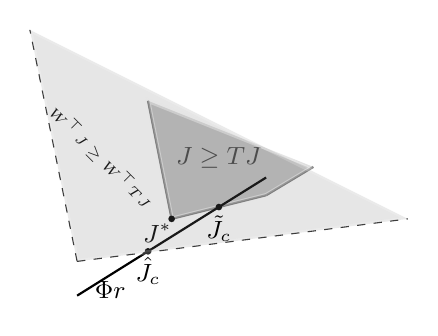
\begin{tikzpicture}[domain=-10:7.7,scale=0.6,font=\small,axis/.style={very thick, ->, >=stealth'}]
%\draw[line,thick,->] (-1,-0.625)--(4,-0.625);
%\draw[line,thick,->] (0,-1)--(0,4);
%\draw[line,thick,-](-0.2,-0.6)--(1,3);
\draw[line,thick,-](0.5,3.5)--(1,1);
\draw[line,thick,-](1,1)--(3,1.5);
\draw[line,thick,-](3,1.5)--(4,2.1);
\node[](one) at (2,2.3){\text{$J\geq TJ$}};
\node[rotate=-45](seven) at (-0.5,2.3){\text{\tiny $W^\top J\geq W^\top TJ$}};
\node[](two) at (-0.3,-0.5){\text{$\Phi r$}};
\node[](three) at (0.7,0.7){\text{$J^*$}};
%\draw[line,thick,-](0,0)--(4,2.5);
 \draw [ultra thick, draw=white, fill=gray, opacity=0.5]
       (0.5,3.5)--(1,1)--(3,1.5)--(4,2.1) -- cycle;
\draw[line,thick,-](-1,-0.625)--(3,1.8750);
 \fill (1,1)  circle[radius=2pt];
 \fill (2,1.25)  circle[radius=2pt];
 \fill (0.5,0.3125)  circle[radius=2pt];
\draw[line,dashed,-](-1,0.1)--(6,1);
\draw[line,dashed,-](-1,0.1)--(-2,5);
 \draw [ultra thick, draw=white, fill=gray, opacity=0.2]
       (-1,0.1)--(6,1)--(-2,5) -- cycle;
\node[] (four) at (2,0.8){\text{$\tilde{J}_c$}};
\node[] (six) at (0.5,-0.1){\text{$\hat{J}_c$}};
\end{tikzpicture}
%}
\caption{The outer lightly shaded region corresponds to GRLP constraints and the inner dark shaded region corresponds to the original constraints. The main contribution of the paper is to bound $||J^*-\hat{J}_c||$.}
\label{cartoon}
\end{figure}


\begin{figure}
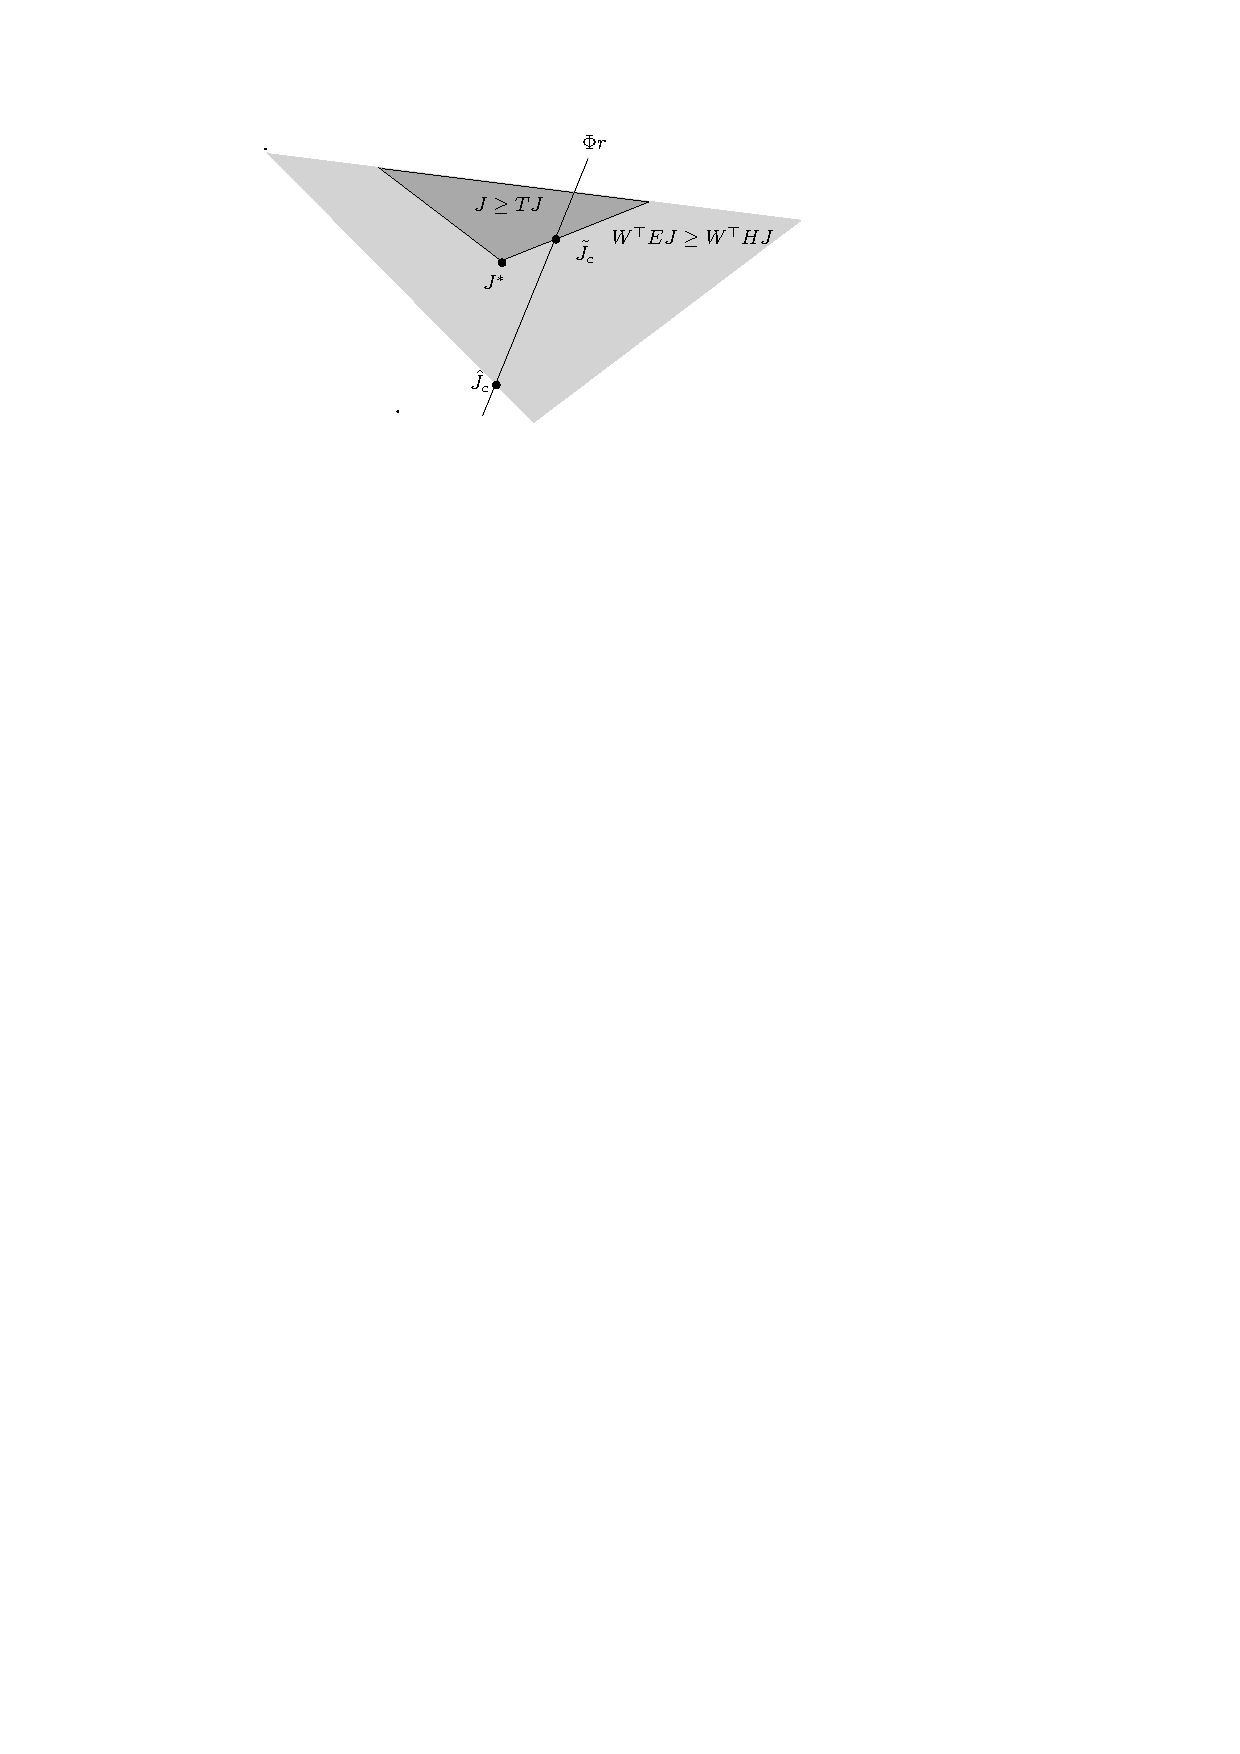
\includegraphics[scale=0.7]{cartoon_grlp.pdf}
\caption{
%\normalsize
The outer lightly shaded region corresponds to GRLP constraints and the inner dark shaded region corresponds to the original constraints. The main contribution of the paper is to bound $\norm{J^*-\hat{J}_c}$.}
\label{cartoon}
\end{figure}
\Cref{cartoon} shows the solutions to the LP, ALP and GRLP respectively. The error in ALP solution has already been studied in \cite{ALP}. Our objective is to study the extra source of error due to constraint approximation.
\section{Main Results}
In this section we present the main results of this paper in \Cref{cmt2} (we state improved bounds in \Cref{sec:improv}). Our bounds are expressed in terms of two novel contractions operators which we define in \Cref{lubpop,alubpop}. We now define two projection operators that are central to our error analysis and in them we assume that the set $\N'\subset \R^k$ is such that $\N' = \N + t \one$ for any $t\in \R$.
%The least upper bound (LUB) projection operator $\Gamma \colon \R^n \ra\R^n$ is defined below, see \eqref{gamdef}.
\begin{definition}\label{lubpop}
Given $J\in \R^n$ and the nonnegative valued vector $c\in \R^n_+$, define $r_{c,J}$ to be the solution to
\begin{align}
\label{lubplp}
\begin{split}
\underset{r\in \N'}{\min} &\,\, c^\top \Phi r\,\mb
\text{s.t.} \mb \Phi r\geq  TJ.
\end{split}
\end{align}
For $J\in \R^n$, $\Gamma J$, the \emph{least upper} (LU) projection of $J$ is defined as
\begin{align}\label{gamdef}
(\Gamma J)(i)\eqdef(\Phi r_{e_i,J})(i),\quad i=1,\ldots,n\,.
\end{align}
\end{definition}
The definition of the second operator is as follows:
\begin{definition}\label{alubpop}
Given $J\in \R^n$ and the nonnegative valued vector $c\in \R^n_+$, define $r'_{c,J}$ to be the solution to
\begin{align}\label{alubplp}
\underset{r\in \N'}{\min}& \,\mb c^\top \Phi r\,\mb
\text{s.t.} \,\,\, W^\top E \Phi r\geq W^\top HJ.
\end{align}
The \emph{approximate least upper} (ALU) projection operator
$\hg \colon \R^n \ra \R^n$ is defined as
\begin{align}\label{tgamdef}
(\hg J)(i)\eqdef(\Phi r'_{e_i,J})(i), \mb i=1,\ldots,n\,, J\in \R^n\,.
\end{align}
\end{definition}
\begin{remark}\label{ubrem}
To understand the meaning of $\Gamma$ (and $\hg$) define
\begin{align}\label{ubclass}
\F_J\eqdef\{\,\Phi r\,:\,\Phi r\geq TJ, r\in \N'\,\},
\end{align}
where $J\in \R^n$.
Disregarding the constraint $r\in \N'$,
$\F_J$ contains all vectors in the span of $\Phi$ that upper bound $TJ$. Further, since $(\Gamma J)(i) = \min\{ V(i) \,:\, V\in \F_J \}$, it also follows that $ V\ge \Gamma J $ holds for any $V\in \F_J$. Also $\Gamma J\geq T J$.\par
The operators $\Gamma$ and $\hg$ are closely related to ALP \eqref{alp} and GRLP \eqref{grlp} respectively and are only analytical tools that we will need to express our bounds and need not be computed in practice. It turns out that the novel operators ($\Gamma$ and $\hg$) are contraction maps (see \Cref{hgmaxcontramn}), a fact that is a key to our results (\Cref{cmt2mn,polthe}). At the outset we are interested in the candidate value functions in the constraint set $\N$ and want to study them using $\Gamma$ and $\hg$. However since the basis $\Phi$ contains $\one$ we make it helps our analysis to define the set $\N'$ in \Cref{lubplp,alubplp} to be `$\N$ plus its translations by $\one$'.
\end{remark}
%\subsection{Error Bounds}
\begin{theorem}[Error Bound for GRLP]
\label{cmt2}
Let $\one\in\R^k$ be in the column span of $\Phi$, then it holds that
\begin{enumerate}
\item The prediction error is bound as\\
$\norm{J^*-\hj}_{1,c}
\leq\frac{1}{1-\alpha}(6~\us{\min}{r\in \R^k}\norm{J^*-\Phi r}_{\infty}
+2\norm{\Gamma J^*-\hg J^*}_{\infty})$.
\item The control error is bound as\\
$\norm{J^* - J_{\hu}}_{1,c}
\leq 2\left(\frac{1}{(1-\alpha)^2}\right)\, \big( 2~\us{\min}{r\in \R^k} \norm{J^*-\Phi r}_{\infty}
+\norm{\Gamma J^*-\hg J^*}_{\infty}+\norm{\hj-\hg\hj}_{\infty}\big)$.
\end{enumerate}
\end{theorem}
\textbf{On Prediction Error:} The first factor in the right hand side of the prediction error in \Cref{cmt2} is related to the best possible approximation that can be achieved with the chosen feature matrix $\Phi$. This term is an carry over of the upper bound in ALP formulation as shown in \Cref{alpvanilla}. The second factor in the right hand side of the prediction error is related to constraint approximation and is completely defined in terms of $\Phi$, $W$ and $T$, and does not require knowledge of stationary distribution of the optimal policy.\par
\textbf{On Control Error:} The first two terms are quite similar to those in the bound for prediction error. The third term occurs due to the fact that $\Phi \geq T\Phi r$ that holds in the case of ALP does not hold in the case of GRLP.\par
\begin{comment}
\begin{theorem}[Control Error Bound in $\norm{\cdot}_{\infty}$]
\label{polthe}
Let $\hu$ be the greedy policy with respect to the solution $\hj$ of GRLP and $J_{\hu}$ be its value function.
% Let $r^*$ be as in Theorem~\ref{mt2mn}, then
Then,
\begin{align}\label{polthebnd}
\norm{J^* - J_{\hu}}_{1,c}
&\leq 2\left(\frac{c^\top \psi}{(1-\beta_{\psi})^2}\right)\, \big( 2\norm{J^*-\Phi r^*}_{\infty}
\nn\\&
+norm{\Gamma J^*-\hg J^*}_{\infty}+\norm{\hj-\hg\hj}_{\infty}\big).
\end{align}
\end{theorem}
\end{comment}
\begin{corollary}[Constraint Sampling]\label{st}
$W\in \{0,1\}^{nd\times m}$Let $s\in S$ be a state whose constraint is selected by $W$ (i.e., for some $i$ and all $(s',a)\in S\times A$,
$W_{s'a,i}=\delta_{s=s'}$.
Then
\begin{align*}%\label{sampexp}
|\Gamma J^*(s)-\hg J^*(s)|<|\Gamma J^*(s)-J^*(s)|.
\end{align*}
\end{corollary}
It is important to note that \Cref{rlpt} holds only in high probability and is valid only under idealized assumption of knowing the optimal policy $u^*$, while \Cref{cmt2} does not have these limitations.
In addition, the error $|\Gamma J^*(s) -\hg J^*(s)|$ (in \Cref{st} ) due to constraint approximation is less than the original projection error $|\Gamma J^*(s)-J^*(s)|$ due to function approximation. This means that for RLP to perform well it is important to retain the constraints corresponding to those states for which the linear function approximation via $\Phi$ is known to perform well.

%!TEX root =  autocontgrlp.tex
\section{Error Analysis}\label{sec:improv}
\subsection{Properties of the Bellman Operator}
We now state without proof the most important properties of the Bellman operator(s).
The proofs are immediate from the definitions, but can also be found in \cite{BertB}.
\begin{comment}
First, we introduce some extra notation:
For $J_1,J_2\in \R^n$, we write $J_1\le J_2$ if $J_1(s)\le J_2(s)$ holds for all $s\in S$.
We use $\one \in \R^n$ to denote a vector with all entries $1$.
The maximum norm $\norm{\cdot}_{\infty}$ is defined by $ \norm{v}_{\infty} = \max_{s\in S} |v(s)|$.
\end{comment}
\begin{lemma}\label{tprop} The following hold:
\begin{enumerate}[(i)]
\item \label{monotone}$T$ is a monotone map, i.e., given $J_1,J_2 \in \R^n$ such that $J_1\leq J_2$, we have $T J_1\leq T J_2$.
\item \label{shift}
Given $J\in \R^n$ and $t \in \R$, we have $T(J+t\one)=TJ+\alpha t\one$.
\item \label{maxnorm}
If $T: \R^n \to \R^n$ is any operator that is monotonous and satisfies~\eqref{shift} then
$T$ is a $\max$-norm contraction operator with contraction factor $\alpha \in (0,1)$, i.e., given $J_1, J_2 \in \R^n$,
$
\norm{TJ_1-TJ_2}_\infty\leq \alpha \norm{J_1-J_2}_\infty.
$
\item \label{uniquesol}
$J^*$ is a unique fixed point of $T$, i.e., $J^*=TJ^*$.
\end{enumerate}
\end{lemma}
\begin{corollary}
If $J\in \R^n$ is such that $J\geq TJ$ then $J\geq TJ^2\geq \ldots \geq J^*$.
\end{corollary}
Though \cref{tprop} are stated for the Bellman operator $T$, the results also hold for $H$ as well.\par
We now present the analysis to derive the improved bounds where the idea is to show that the novel projection operators ($\Gamma/\hg$) are contraction maps. To this end, we go through steps similar to \Cref{tprop}-\eqref{monotone},~\eqref{shift} and ~\eqref{maxnorm}. Much the results that ensue are based on `Lyapunov' analysis where the idea is to replace the constant function $\one$ by a certain Lyapunov function (see \Cref{def:lyap}) and the $\norm{\cdot}_{\infty}$ by a weighted max-norm (see \Cref{notations}-\eqref{norms}).
\subsection{Analysis using Lyapunov Functions}
\begin{definition}\label{def:lyap}
Let $c,\rho,\chi:S \to \R_+$ be positive-valued functions. Then for $J\in \R^n$, $a\in A$ and $s\in S$, define
the discounted maximal inflation of $\chi$ due to $P = (p_a)_{a\in A}$ as $\beta_{\chi}=\max_{s \in S} \frac{\underset{a \in A}{\max}\big(\alpha\sum_{s'}p_a(s,s')\chi(s')\big)}{\chi(s)}$.
The function $\chi:S\to\R_+$ is a \emph{Lyapunov} function for $P = (p_a)_{a\in A}$ if $\beta_{\chi}<1$.
\end{definition}
\begin{assumption}\label{grlpassmp}
\begin{enumerate}[(i)]
%\item \label{one} The first column of the feature matrix $\Phi$ (i.e., $\phi_1$) is $\one \in \R^n$.
\item \label{lyap} $\psi\colon S \ra \R_+$ is a Lyapunov function for $P$
and is present in the column span of the feature matrix $\Phi$: For some $r_0\in \R^k$, $\Phi r_0 = \psi$.
\item \label{ass:n4} The set $\N'$ is such that $\N' = \N + t r_0$ for any $t\in \R$, where $r_0\in \R^k$ such that $\Phi r_0 = \psi$.
\item \label{wassmp} $W \in \R^{nd\times m}_+$ is a matrix with all positive entries.
\end{enumerate}
\end{assumption}
The authors of \cite{ALP} express the error bounds in terms of $\frac{1}{1-\beta_{\psi}}$.  A smaller $\beta_{\psi}$ loosely implies `stability' of the the underlying MDP,  with smaller values representative of higher stability. Prior works in ALP literature \cite{ALP,SALP,CS} make use of Lyapunov functions based analysis to obtain error bounds that exploit the structure of the underlying MDP. In particular, the prior bounds suggests that the ALP is likely to generate good approximations when the underlying MDP is stable. We also adopt a similar approach by stating our results using Lyapunov function based arguments.

We note in passing that if \cref{grlpassmp}-\eqref{lyap} holds, it follows that for any $J\in \R^n$ and $t>0$,
\begin{align}\label{eq:psilin}
\begin{split}
T(J+ t \psi ) \le TJ + \beta_{\psi}\,t\,  \psi,\\
H(J+ t \psi ) \le HJ + E \beta_{\psi}\,t\,  \psi\,.
\end{split}
\end{align}
%\begin{figure}[h!]
\centering
%\resizebox{columnwidth}{}{
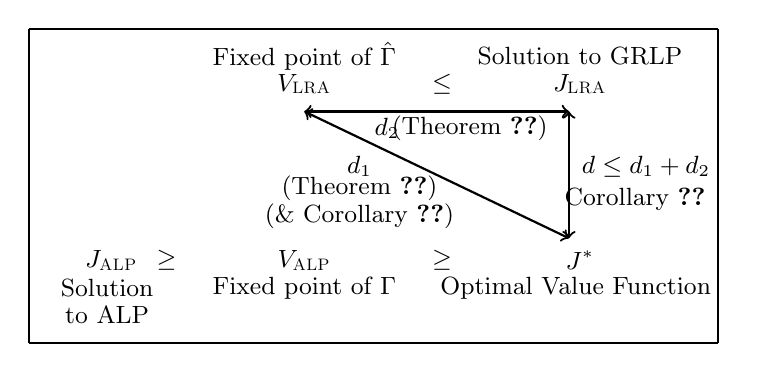
\begin{tikzpicture}[domain=0:7.7,scale=0.7,font=\small,axis/.style={very thick, ->, >=stealth'}]
\draw [line,thick,-] (0,-1)--(0,4.7);
\draw [line,thick,-] (0,4.7)--(12.5,4.7);
\draw [line,thick,-] (12.5,4.7)--(12.5,-1);
\draw [line,thick,-] (0,-1)--(12.5,-1);
\node[](one) at (1.5,0.5) {$\tj$};
\node[](four) at (2.5,0.5) {$\geq$};
\node[](two) at (5,0.5) {$\tv$};
\node[](three) at (10,0.5) {$J^*$};
\node[](five) at (7.5,0.5) {$\geq$};
\node[](six) at (10,3.7) {$\hj$};
\node[](seven) at (5,3.7) {$\hv$};
\node[](eight) at (7.5,3.7) {$\leq$};
\node[](nine) at(1.5,0){\text{Solution }};
\node[](twenty) at(1.5,-0.5	){\text{to ALP }};
\node[](ten) at(5,0){\text{Fixed point of }$\Gamma$};
\node[](eleven) at(10,0){\text{Optimal Value Function }};
\node[](twelve)at (10,4.2){\text{Solution to GRLP}};
\node[](thirteen)at (5,4.2){\text{Fixed point of }$\hg$};
\draw [line,thick,<->] (5,3.2)--(9.8,0.9);
\draw [line,thick,<->] (5,3.2)--(9.8,3.2);
\draw [line,thick,<->] (9.8,3.2)--(9.8,0.9);
\node[](fourteen)at (6,2.2){$d_1$};
\node[](fifteen)at (6.5,2.9){$d_2$};
\node[](sixteen)at (11.2,2.2){$d\leq d_1+d_2$};
\node[](eighteen)at (11,1.6){\text{Corollary~\ref{cmt2}}};
\node[](seventeen)at (8,2.9){\text{(Theorem~\ref{mt2}})};
\node[](fourteen)at (6,1.8){\text{(Theorem~\ref{mt1})}};
\node[](fourteen)at (6,1.3){\text{(\& Corollary~\ref{cmt1})}};
%\node[rotate=-25](fourteen)at (7.5,1.5){\text{(Theorem~\ref{mt1})}};
%\node[draw, circle](two) at (5.5,1) {$s_{n+1}=s'$};
%\draw[->, =>latex](one) edge[bend left=42.5](two);
%\node [above=1.1cm]at (2.8,1.2) {${p_{a_n}(s,s')}$};
%\node [right] at(0,0){$g_{a_n}(s_n)$};
\end{tikzpicture}
%}
\caption{A schematic of the error analysis. Here $d=||J^*-\hj||_{1,c}.$}
\label{schematic}
\end{figure}


The next lemma is elementary, but will prove to be useful:
\begin{lemma}\label{lpsol}
Let $A\in \R^{u\times v}$, $b\in \R^u,d\in \R^v$ and $b_0=Ax_0$ for
some $x_0 \in \R^v$, $\N' \subset \R^v$ such that $\N' =x_0+ \N'$. Then
\begin{align}
&\min\{d^\top x:Ax\geq b+b_0, x\in \N'\} \nn\\
&=\min\{d^\top y:Ay \geq b, y \in \N' \}+d^\top x_0.
\end{align}
\end{lemma}
\begin{proof}
The claim follows by the change of variables $y := x-x_0$.
\end{proof}
\noindent 
%Note that under our assumptions on $\N$, $\hg$ is well-defined.
%\begin{align*}
%r^*\eqdef\argmin_{r\in R^k}\norm{J^*-\Phi r}_{\mn}\,.
%\end{align*}
%where $\psi$ is a Lyapunov function as in \cref{lyap}.
\begin{lemma}\label{bestbndmn}
Let $r^*\eqdef\underset{r\in \R^k}{\min}\parallel J^*-\Phi r\parallel_{\mn}$. Then,
\begin{align}
\norm{J^*-\Gamma J^*}_{\mn}\leq 2 \norm{J^*-\Phi r^*}_{\mn}.
\end{align}
\end{lemma}
\begin{proof}
Define $\eps = \norm{J^* - \Phi r^*}_{\mn}$ so that
$ J^*-\Phi r^* \le \eps \psi$ and $\Phi r^* - J^*\le \eps \psi$. Then, from \cref{grlpassmp}-\eqref{ass:n4} it follows that $\Phi( r^* + \eps r_0 ) = \Phi r^* + \eps \psi \ge J^* = T J^*$. From the definition of $\Gamma$ in \eqref{gamdef} and \cref{ubrem}, we know that $\Phi r^*+\eps \psi \geq \Gamma J^*\geq J^*$. The result follows by noting that $2\eps\psi\geq \Phi r^*+\eps\psi -J^*\geq \Gamma J^*-J^*\geq 0$.
\end{proof}
\begin{lemma}\label{tgmonotone}
For $J_1, J_2\in \R^n$ such that $J_1\leq J_2$, we have $\hg J_1\leq \hg J_2$.
\end{lemma}
\begin{proof}
Given $J\in \R^n$, let $\F_J\eqdef\{\,\Phi r\,: W^\top E \Phi r\geq W^\top HJ, r\in \N'\,\}\,$. Choose any $i\in \{1, \ldots, n\}$. Since $J_1\leq J_2$, from \Cref{tprop}-\eqref{monotone} and \cref{grlpassmp}-\eqref{wassmp} it follows that $W^\top H J_1\leq W^\top H J_2$. Hence, $\F_{J_2} \subset \F_{J_1}$ and thus $(\hg J_1)(i) \le (\hg J_2)(i)$.  Since $i$ was arbitrary, the result follows.
\end{proof}
\begin{lemma}\label{maxnormmn}
Assume that $\hg: \R^n \to \R^n$ is monotone and 
that there exists some $\beta\in [0,1)$ such that for any $J\in \R^n$ and $t>0$,
\begin{align}
\label{eq:shiftmn}
\hg( J + t \psi) \le \hg J + \beta t \psi.
\end{align} 
Then $\hg$ is a $\norm{\cdot}_{\mn}$ contraction with factor $\beta$.
\end{lemma}
\begin{proof}
First, we show that for any $t\ge 0$,  $J\in \R^n$,
$\hg( J - t \psi) \ge \hg J - \beta t \psi$ also holds.
To see this define $J' = J-t\psi$. Then, $J = J'+t\psi$, hence $\hg J \le \hg J' + \beta t \psi$. Reordering this inequality gives the result.
Let $\eps = \norm{J_1 - J_2}_{\mn}$, where $J_1,J_2\in \R^n$ are arbitrary.
Then $J_2 - \eps \psi \le J_1 \le J_2 + \eps \psi$. 
By the monotonicity of $\hg$,
$\hg(J_2 - \eps \psi) \le \hg J_1 \le \hg(J_2 + \eps \psi)$. 
Using~\eqref{eq:shiftmn}, we get 
$\hg J_2 - \beta \eps \psi \le \hg J_1 \le \hg J_2 + \beta \eps \psi$, i.e., $-\beta \eps \psi \le \hg J_1 - \hg J_2 \le \beta \eps \psi$, from which the result follows.
\end{proof}
\begin{corollary}\label{tmaxnormmn}
$T$ is a $\norm{\cdot}_{\mn}$-contraction with factor $\beta_{\psi}$.
\end{corollary}
%Returning to $\hg$, since we already now that $\hg$ is monotone (cf. \cref{gmonotone}), it remains to see that it satisfies \eqref{eq:shiftmn}:
\begin{lemma}\label{gshiftmn}
The operator $\hg$ satisfies \eqref{eq:shiftmn} with $\beta = \beta_\psi$.
%For any $J\in \R^n$, $t\in \R_+$, $\Gamma (J+ t \psi ) \le \Gamma J + \beta_{\psi} t \psi$.
\end{lemma}
\begin{proof}
By definition, for $1\le i \le n$, $(\hg (J+t\psi) )(i) = \min\{ e_i^\top \Phi r \,:\, W^\top E\Phi r \ge W^\top H(J+t\psi), r\in \N' \}$.
By \eqref{eq:psilin}, as $t>0$, $H(J+t\psi) \le HJ + t \beta_\psi \psi$ and hence $W^\top H(J+t\psi) \le W^\top (HJ + t \beta_\psi \psi)$. Thus,
$(\hg (J+t\psi) )(i) \le 
 \min\{ e_i^\top \Phi r \,:\, W^\top E\Phi r \ge W^\top HJ+t\beta_\psi \psi), r\in \N' \}$.
Now, using \Cref{lpsol} with $A=W^\top E \Phi$, $b=W^\top HJ$, $d=e_i\Phi$, $b_0=t\beta_\psi \psi$
and $x_0=t \beta_\psi r_0$, the statement follows since $A x_0 = b_0$ (from \cref{grlpassmp}-\eqref{lyap}) and $\N' = \N' + \alpha t r_0$ (from \cref{grlpassmp}-\eqref{ass:n4}).
\end{proof}
%From this result and \cref{maxnormmn}, we immediately get that $\Gamma$ is a contraction in $\norm{\cdot}_{\mn}$:
\begin{comment}
\begin{theorem}\label{gmaxcontramn}
The operator $\Gamma  \colon \R^n\ra \R^n$ is a contraction operator in $\norm{\cdot}_{\mn}$ with factor $\beta_{\psi}$.
\end{theorem}
\end{comment}
%In a similar way, one can also show that $\hg$ is also a contraction:
\begin{theorem}\label{hgmaxcontramn}
The operator $\hg:\R^n\to\R^n$  is a contraction operator in $\norm{\cdot}_{\mn}$ with factor $\beta_{\psi}$.
%$\hg$ is also a contraction map in the weighted $L_\infty$ norm.
\end{theorem}
\begin{proof}
Follows from \cref{maxnormmn,gshiftmn}.
\begin{comment}
We already know that $\hg$ is monotone. That $\hg$ satisfies~\cref{eq:shiftmn}
with $\beta = \beta_{\psi}$ follows similarly to the argument used in  \cref{tgshift}
with modifications similar to those introduced in the proof of \cref{gshiftmn}.
Then, \cref{gmaxcontramn} gives the desired result.
\end{comment}
\end{proof}
In what follows we denote by $\hv$ the unique fixed point of $\hg$, i.e., $\hv = \hg \hv\,$. 
We now show that vector $\hj$ dominates $\hv$:
\begin{lemma}\label{relation1}
The vectors $\hv,\hj$ obey $\hj\geq\hv$.
\end{lemma}
\begin{proof}
For $i\in \{1,\dots,n\}$, $c=e_i$ let $r_i$ be a solution to the GRLP in \eqref{grlp}
and define $V_0\in \R^n$ by $V_0(i)=\underset{j=1,\ldots,n}{\min}(\Phi r_j)(i)$, $1\le i \le n$.

It suffices to show that $V_1\eqdef \hg V_0 \le V_0 \le \hj$ since then the desired result follows
by defining $V_{n+1} = \hg V_n$, $n\ge 1$, noting that by \cref{tgmonotone}, $V_{n+1}\le V_{n}$ and by  \cref{tmaxnormmn}, $V_n \to \hv$.

Since $(\Phi r_j)(i) \ge (\Phi r_i)(i)$ also holds for any $1\leq i,j\leq n$ we have $V_0(i)  = (\Phi r_i)(i)$. Also, since $\hj(i) \ge (\Phi r_i)(i),1\leq i \leq n$ it follows that $\hj\geq V_0$. 
Now,  fix any $i$. 
We need to show that $V_1(i)=(\hg V_0)(i) = (\Phi r'_{e_i,V_0})(i) \leq V_0(i)$. 
By the definition of $r'_{e_i,V_0}$ we know that $(\Phi r'_{e_i,V_0})(i) \le (\Phi r)(i)$
holds for any $r\in \N$ such that $W^\top E \Phi r \ge W^\top H V_0$. 
Now it suffices to show that $r_i$ satisfies $W^\top E \Phi r_i \ge W^\top H V_0$. 
By definition, $r_i$ satisfies $W^\top E \Phi r_i \ge W^\top H \Phi r_i$.
Hence, by the monotone property of $H$ and \cref{grlpassmp}-\eqref{wassmp} it is sufficient if $\Phi r_i \ge V_0$.
This however follows from the definition of $V_0$.
\end{proof}
\begin{lemma}\label{relation2}
The vectors $\hv,\tj$ obey $\tj\geq\hv$.
\end{lemma}
\begin{proof}
%The proof follows in a similar manner as the proof of \Cref{relation1}. To elaborate, 
Let $ r_1,  r_2,\ldots, r_n$ be solutions to the ALP in \eqref{alp} (with an additional constraint that the solution be restricted to $\N$) for $c=e_1, e_2,\ldots,e_n$, respectively,
and define $V_0\in \R^n$ by $V_0(i)=\underset{j=1,\ldots,n}{\min}(\Phi r_j)(i)$, $1\le i \le n$. The rest of the proof 
follows in the same manner as the proof of \cref{relation1}.
\end{proof}
\begin{lemma}\label{srw}
A vector
$\hat{r} \in \R^k$ is a solution to GRLP \eqref{grlp} iff it solves the following program:
\begin{align}\label{grlpeqprog}
\begin{split}
\min_{r\in \N}\, &\norm{\Phi r-\hv}_{1,c}\,\mb
\text{s.t.}\mb \, W^\top E \Phi r\geq W^\top H \Phi r.
\end{split}
\end{align}
\end{lemma}
\begin{proof}
We know from \Cref{relation1} that $\hj = \Phi \hr \geq\hv$, and thus
the solutions to \eqref{grlp} do not change if we add the constraint $\Phi r \ge \hv$.
Now, under this constraint, minimizing $c^\top \Phi r$ is the same as minimizing 
\begin{align*}
\norm{\Phi r-\hv}_{1,c}=\sum_{i=1}^n c(i) |(\Phi r)(i)-\hv(i)|=c^\top \Phi r-c^\top \hv\,.
\end{align*} 
\end{proof}
\begin{lemma}\label{srwalp}
A vector
$\tr \in \R^k$ is a solution to ALP \eqref{alp} iff it solves the following program:
\begin{align}\label{grlpeqprog}
\begin{split}
\min_{r\in \R^k}\, &\norm{\Phi r-\hv}_{1,c}\,\mb
\text{s.t.}\mb \, \Phi r\geq  T \Phi r.
\end{split}
\end{align}
\end{lemma}
\begin{proof}
We know from \Cref{relation2} that $\tj = \Phi \tr \geq\hv$.
The rest of the argument follows in the same manner as the proof for \cref{srw}.
\end{proof}
\begin{lemma}\label{cmt1mn}
We have
\begin{align}
\norm{J^*-\hv}_{\mn}
& \leq \frac{1}{{1-\beta_{\psi}}}\big(2\norm{J^*-\Phi r^*}_{\mn}
\nn\\
& {}\qquad \qquad+\norm{\Gamma J^*-\hg J^*}_{\mn}\big).
\end{align}
\end{lemma}
\begin{proof}
Recall that $\hg \hv=\hv$. By the triangle inequality,
\begin{align*}
\norm{J^*-\hv}_{\mn}
& \leq \norm{J^*-\hg J^*}_{\mn}+\norm{\hg J^*-\hg \hv}_{\mn}\\
&\leq \norm{J^*-\hg J^*}_{\mn}+\beta_\psi \norm{ J^*- \hv}_{\mn},
\end{align*}
and so by reordering and with another triangle inequality,
\begin{align}\label{jhv}
\norm{J^*-\hv}_{\mn} \nn
&\le \frac{\norm{ J^*-\hg J^*}_{\mn}}{1-\beta_\psi}\nn\\
&\le \frac{\norm{ J^*-\Gamma J^*}_{\mn}+\norm{\Gamma J^* - \hg J^*}_{\mn}}{1-\beta_\psi}\,.
\end{align}
The proof follows by combining this and \cref{bestbndmn}.
\end{proof}
We now recall Lemma~$5$ from Section 4.2 of \cite{ALP}. 
For this result, recall that $r_0 \in \R^k$ is the vector such that $\psi = \Phi r_0$.
\begin{lemma}\label{restate}
%Let $\psi$ be a Lyapunov function that belongs to the column span of $\Phi$ ,
For  $r \in \R^k$ arbitrary, let $r'$ be
\begin{align}
r'= r+\norm{J^*-\Phi r}_{\mn} \left(\frac{1+\beta_{\psi}}{1-\beta_{\psi}}\right)\, r_0.
\end{align}
Then $r'$ is feasible for the ALP in \eqref{alp}.
\end{lemma}
Recall that $\hv$ is the fixed point of $\hg$ and $\hj=\Phi \hr$ is the solution to the GRLP
\eqref{grlp}. 
\begin{theorem}\label{mt2mn}
We have
\begin{align}
\norm{\hj-\hv}_{1,c}&\leq \frac{c^\top \psi}{1-\beta_\psi}(4\norm{J^*-\Phi r^*}_{\mn}\nn
+\norm{\Gamma J^*-\hg J^*}_{\mn}).
\end{align}
\end{theorem}
\begin{proof}
Let $\gamma=\norm{J^*-\Phi r^*}_{\mn}$.
Then, by choosing $r'$ as in \Cref{restate} we have
\begin{align}
\norm{\Phi r'-J^*}_{\mn}\nn
&\leq \norm{\Phi r^*-J^*}_{\mn}+\norm{\Phi r'-\Phi r^*}_{\mn}\nn\\
&=\gamma+\frac{1+\beta_\psi}{1-\beta_\psi}\gamma
	=\frac{2}{1-\beta_\psi}\gamma.
\label{part}
\end{align}
%We know that $\tr \in \N$ by \cref{grlpassmp}-\eqref{nassmp} and 
Now, $r'$ is feasible for the ALP in \eqref{alp} by \cref{restate}.
Then from \cref{srwalp} it follows that
%As a result, from \cref{srw} it follows that
\begin{align}
\norm{\hj-\hv}_{1,c}
&\leq\norm{\Phi \tr-\hv}_{1,c}\leq\norm{\Phi r'-\hv}_{1,c}\nn\\
&=\sum_{s\in S}c(s)\psi(s)\frac{|\Phi r'(s)-\hv(s)|}{\psi(s)}\nn\\
&\leq c^\top \psi \norm{\Phi r'-\hv}_{\mn}\nn\\
&\leq c^\top \psi (\norm{\Phi r'-J^*}_{\mn}+\norm{J^*-\hv}_{\mn}).\nn
\end{align}
The result follows from \cref{cmt1mn} and \eqref{part}.
%\textbf{Main Result~$1$: Prediction Error bound in weighted $L_\infty$-norm}
\end{proof}
\begin{theorem}[Prediction error bound]
\label{cmt2mn}
%Let $\hj$, $\hv$, $r^*$ and $J^*$ be as in Theorem~\ref{mt2mn}, then
It holds that
\begin{align}\label{finalbndmn}
\begin{split}
\norm{J^*-\hj}_{1,c}
&\leq\frac{c^\top\psi}{1-\beta_\psi}(6 \norm{J^*-\Phi r^*}_{\mn}\\
&+2\norm{\Gamma J^*-\hg J^*}_{\mn}).
\end{split}
\end{align}
\end{theorem}
\begin{proof}
We have
\begin{align}
\norm{J^*-\hj}_{1,c}\nn
&\leq\norm{J^*-\hv}_{1,c}+\norm{\hv-\hj}_{1,c}\nn\\
&\leq c^\top \psi \norm{J^*-\hv}_{\mn}+\norm{\hv-\hj}_{1,c}.\nn
\end{align}
The result now follows from \Cref{cmt1mn} and \Cref{mt2mn}.
\end{proof}
We now bound the performance of the greedy policy $\hu$.
\begin{theorem}[Control Error Bound]
\label{polthe}
Let $\hu$ be the greedy policy with respect to the solution $\hj$ of the GRLP and $J_{\hu}$ be its value function.
% Let $r^*$ be as in Theorem~\ref{mt2mn}, then
Then,
\begin{align}\label{polthebnd}
\norm{J^* - J_{\hu}}_{1,c}
&\leq 2\left(\frac{c^\top \psi}{(1-\beta_{\psi})^2}\right)\, \big( 2\norm{J^*-\Phi r^*}_{\mn}
\nn\\&
+\norm{\Gamma J^*-\hg J^*}_{\mn}+\norm{\hj-\hg\hj}_{\mn}\big).
\end{align}
\end{theorem}
\begin{proof}
By the triangle inequality,
\begin{align*}
\norm{J^*-J_{\hu}}_{1,c}&\leq \norm{J^*-\hj}_{1,c}+\norm{J_{\hu}-\hj}_{1,c}\,.
\end{align*}
Let us now bound the second term on the right-hand side.
Since $\hu$ is greedy w.r.t. $\hj$, it holds that $T_{\hu} \hj = T \hj$.
Also, $T_{\hu} J_{\hu} = J_{\hu}$.
Hence, $J_{\hu} - \hj = T_{\hu} J_{\hu} - T_{\hu} \hj + T \hj - \hj
=\alpha P_{\hu} (J_{\hu}- \hj) + T\hj - \hj$.
Hence,
\begin{align}\label{polderv}
||J_{\hu}-\hj||_{1,c}\nn
&=||(I-\alpha P_{\hu})^{-1}(T\hj-\hj)||_{1,c}\nn\\
&\leq c^\top(I-\alpha P_{\hu})^{-1}|T\hj-\hj|\nn\\
&\leq c^\top (I-\alpha P_{\hu})^{-1} \,\psi\, \norm{T\hj-\hj}_{\mn}\nn\\
&\leq \frac{c^\top \psi}{1-\beta_{\psi}}\norm{T\hj-\hj}_{\mn}\nn\\
%&\leq \frac{c^\top \psi}{1-\beta_{\psi}}\norm{T\hj-TJ^* +J^*- \hj}_{\mn}\nn\\
&\leq \frac{c^\top \psi}{1-\beta_{\psi}}(\norm{T\hj-TJ^*}_{\mn} +\norm{J^*- \hj}_{\mn})\nn\\
&\leq \frac{c^\top \psi}{1-\beta_{\psi}}(1+\beta_{\psi})\norm{J^*- \hj}_{\mn},
\end{align}
where in the second inequality, we use Jensen's inequality and $|T\hj - \hj|$ stands for the 
vector whose $i$th component is $|(T\hj)(i) - \hj(i)|$. Further, the last inequality follows
since $T$ is a $\norm{\cdot}_{\mn}$ contraction with factor $\beta_{\psi}$ as noted earlier.
%componentwise  $(I-\alpha P_{\hu})^{-1}$ is a positive operator for $x=(x_1,\ldots,x_n)^\top\in \R^n$, $|x|=(|x_1|,\ldots,|x_n|)^\top\in \R^n$. 
Hence,
\begin{align}
&\norm{J^*-J_{\hu}}_{1,c}\nn\\
%&\leq \norm{J^*-\hj}_{1,c}+\norm{J_{\hu}-\hj}_{1,c}\nn\\
&\leq c^\top \psi \norm{J^*-\hj}_{\mn}+c^\top \psi\frac{1+\beta_\psi}{1-\beta_\psi}\norm{J^*- \hj}_{\mn}\nn\\
&=\frac{2c^\top \psi}{1-\beta_{\psi}}\norm{J^*- \hj}_{\mn}.
\end{align}
Now in a manner similar to \cref{cmt2mn} we have
\begin{align}
\norm{J^*- \hj}_{\mn}&\leq \norm{J^*- \hv}_{\mn}+\norm{\hv -\hj}_{\mn}\nn
\end{align}
The result now follows by substituting the bound on $\norm{J^*- \hv}_{\mn}$ from \cref{cmt1mn} and the fact that $\norm{\hv-\hj}_{\mn}\leq \frac{1}{1-\beta_{\psi}}\norm{\hj-\hg\hj}_{\mn}$.
\end{proof}
\begin{comment}
\begin{note}
By bounding $\etmn=\norm{\Gamma J^*-J^*+J^*-\hg J^*}_{\mn}\leq 2\norm{J^*-\Phi r^*}_{\mn}+\norm{J^*-\hg J^*}_{\mn}$
(the inequality follows from \cref{bestbndmn}), 
we can loosen the bounds in \cref{cmt2mn} and \cref{polthe} to
\begin{align}
\label{loose1}
\norm{J^*-\hj}_{1,c}&\leq\frac{c^\top\psi}{1-\beta_\psi}(10 \norm{J^*-\Phi r^*}_{\mn}
\nn\\&
+2\norm{J^*-\hg J^*}_{\mn}).\\
\label{loose2}
\norm{J^* - J_{\hu}}_{1,c}&\leq 2\left(\frac{c^\top \psi}{1-\beta_{\psi}}\right)^2 \,\big(10 \norm{J^*-\Phi r^*}_{\mn}
\nn\\&
+2\norm{J^*-\hg J^*}_{\mn}\big).
\end{align}
Here the term $||J^*-\hg J^*||$ in \eqref{loose1} and \eqref{loose2} captures the error due to the use of both $\Phi$ and $W$. Though, \eqref{loose1} and \eqref{loose2} might be loser bounds than \eqref{finalbndmn} and \eqref{polthebnd} respectively, the advantage of this bound is that it captures the error due to function approximation as well as constraint reduction in a direct manner.
\end{note}
\end{comment}
\begin{theorem}[Constraint Sampling]
Let $s\in S$ be a state whose constraint is selected by $W$ (i.e., for some $i$ and all $(s',a)\in S\times A$,
$W_{s'a,i}=\delta_{s=s'}$.
Then
$
|\Gamma J^*(s)-\hg J^*(s)|<|\Gamma J^*(s)-J^*(s)|.
$
\end{theorem}

\begin{proof}
Let $r_{e_s,J^*}$ and ${r}'_{e_s,J^*}$ be solutions to the linear programs in \eqref{lubplp} and \eqref{alubplp} respectively for $c=e_s$ and $J=J^*$. It is easy to note that $r_{e_s,J^*}$ is feasible for the linear program in \eqref{alubplp} for $c=e_s$ and $J^*$, and hence it follows that $(\Phi r_{e_s,J^*})(s)\geq (\Phi {r}'_{e_s,J^*})(s)$. However, since the constraints with respect to state $s$ have been chosen we know that $(\Phi {r}'_{e_s,J^*})(s)\geq J^*(s)$. The proof follows from noting that $(\Gamma J^*)(s)=(\Phi r_{e_s,J^*})(s)$ and $\hg J^*(s)=(\Phi {r}_{e_s,J^*})(s)$.
\end{proof}




%!TEX root =  autocontgrlp.tex
\subsection{Discussion}
\begin{comment}
The error bounds in the main results (Theorems~\ref{cmt2mn} and \ref{polthe}) contain two factors, namely
\begin{enumerate}
\item $\min_{r\in \R^k} ||J^*-\Phi r||_{\mn}$, and
\item $||\Gamma J^*-\hg J^*||_{\mn}$.
\end{enumerate}
The first factor is related to the best possible approximation that can be achieved with the chosen feature matrix $\Phi$. This term is inherent to the ALP formulation and it appears in the bounds provided by \cite{ALP}.\par
The second factor is related to constraint approximation and is completely defined in terms of $\Phi$, $W$ and $T$, and does not require knowledge of stationary distribution of the optimal policy. It makes intuitive sense since given that $\Phi$ approximates $J^*$, it is enough for $W$ to depend on $\Phi$ and $T$ without any additional requirements.\par An interesting feature is that unlike prior work on constraint sampling based on concentration inequalities (e.g.,  \cite{CS}), our analysis is based on contraction operators and is completely deterministic.
In particular, the error term $\etmn$ gives new insights into constraint selection:
\begin{theorem}\label{st}
Let $s\in S$ be a state whose constraint is selected by $W$ (i.e., for some $i$ and all $(s',a)\in S\times A$, 
$W_{s'a,i}=\delta_{s=s'}$. 
Then
\begin{align}\label{sampexp}
|\Gamma J^*(s)-\hg J^*(s)|<|\Gamma J^*(s)-J^*(s)|.
\end{align}
\end{theorem}
\end{comment}
\begin{proof}
Let $r_{e_s,J^*}$ and ${r}'_{e_s,J^*}$ be solutions to the linear programs in \eqref{lubplp} and \eqref{alubplp} respectively for $c=e_s$ and $J=J^*$. It is easy to note that $r_{e_s,J^*}$ is feasible for the linear program in \eqref{alubplp} for $c=e_s$ and $J^*$, and hence it follows that $(\Phi r_{e_s,J^*})(s)\geq (\Phi {r}'_{e_s,J^*})(s)$. However, since the constraints with respect to state $s$ have been chosen we know that $(\Phi {r}'_{e_s,J^*})(s)\geq J^*(s)$. The proof follows from noting that $(\Gamma J^*)(s)=(\Phi r_{e_s,J^*})(s)$ and $\hg J^*(s)=(\Phi {r}_{e_s,J^*})(s)$.
\end{proof}
\begin{comment}
The expression in \eqref{sampexp} in Theorem~\ref{st} says that the additional error $|\Gamma J^*(s) -\hg J^*(s)|$ due to constraint approximation is less than the original projection error $|\Gamma J^*(s)-J^*(s)|$ due to function approximation. This means that for the RLP to perform well it is enough to retain those states for which the linear function approximation via $\Phi$ is known to perform well. The modified $L_\infty$ norm in \eqref{finalbndmn} comes to our rescue to control the error due to those states that are not chosen.
\end{comment}

%!TEX root =  autocontgrlp.tex
\section{Numerical Illustration}
In this section, we show via an example in the domain of controlled queues that the error term $\et$ indeed correlates with
 the error induced by the constraint approximation. The queuing model used here is similar to the one in Section~$5.2$ of \cite{ALP}. We consider a single queue with arrivals and departures. The state of the system is the queue length with the state space given by $S=\{0,\ldots,n-1\}$, where $n-1$ is the buffer size of the queue. The action set $A=\{1,\ldots,d\}$ is related to the service rates. We let $s_t$ denote the state at time $t$. The state at time $t+1$ when action $a_t \in A $ is chosen is given by $s_{t+1}= s_{t}+1$ with probability $p$, $s_{t+1}= s_{t}-1$ with probability $q(a_t)$ and $s_{t+1}= s_t$, with probability $(1-p-q(a_t))$. For states $s_t=0$ and $s_t=n-1$, the system dynamics is given by 	$s_{t+1}= s_{t}+1$ with probability $p$ when $s_t=0$ and $s_{t+1}=s_t-1$ with probability $q(a_t)$ when $s_t=n-1$. The service rates satisfy $0<q(1)\leq \ldots\leq q(d)<1$ with $q(d)>p$ so as to ensure `stabilizability' of the queue. The reward associated with the action $a \in A$ in state $s\in S$ is given by $g_a(s)=-(s+60q(a)^3)$. We made use of polynomial features in $\Phi$ (i.e., $1,s,\ldots,s^{k-1}$) since they are known to work well for this domain \cite{ALP}.
For our experiments, we chose two contenders for the $W$-matrix and compared them with random positive matrices $W_r$. Our choices of the $W$ matrix were: {$\mathbf{(i)}$} $W_c$- matrix that corresponds to sampling according to $c$. This is justified by the insights obtained from Theorem~\ref{st} on the error term $\et$, i.e., the idea of selecting the important states. {$\mathbf{(ii)}$} $W_a$ state-aggregation matrix, a heuristic derived using the fact that $\lambda^*$ is a linear combination of $\{P_{u^*},P^2_{u^*},\ldots\}$. Our choice of the $W_a$ matrix to correspond to aggregation of nearby states is motivated by the observation that $P^n$ captures $n^{th}$ hop connectivity/neighborhood information. 
The aggregation matrix $W_a$ is defined as below: for all $ i=1,\ldots,m$,
\begin{align}\label{wdes}
W_a(i,j)&=1, \mb\text{for all } j\mb\text{s.t.}\mb \nn\\&j=(i-1)\times\frac{n}{m}+k+(l-1)\times n, \nn\\&\mb\quad\quad k=1,\ldots,\frac{n}{m}, l=1,\ldots,d,\nn\\
&=0,\mb\text{otherwise}.
\end{align}
We ran our experiments on a moderately large queuing system denoted by $Q_L$ with $n=10^4$ and $d=4$ with $q(1)=0.2$, $q(2)=0.4$, $q(3)=0.6$, $q(4)=0.8$, $p=0.4$ and $\alpha=0.98$. We chose $k=4$ (i.e., we used $1, s,s^2$ and $s^3$ as basis vectors) and we chose $W_a$ \eqref{wdes}, $W_c$, $W_i$ and $W_r$ with $m=50$, where $W_i$ is the ideal 
(and intractable) sampler of \citep{CS}.
We set $c(s)=(1-\zeta) \zeta^s$, where $s=1,\ldots,9999$, with $\zeta=0.9$ and $\zeta=0.999$ respectively. The results in Table~\ref{pref} show that the performance exhibited by $W_a$ and $W_c$ is better by several orders of magnitude over `random' in the case of the large system $Q_L$ and is closer to the ideal sampler $W_i$. Note that computing $\et$ was hard in the case of large $n=10^4$ and since $\et$ is completely dependent on the structure of $\Phi$, $T$ and $W$ we instead computed the same for $n=10$ and used it as a surrogate. Accordingly, we chose a smaller system $Q_S$ with $n=10$, $d=2$, $k=2$, $m=5$, $q(1)=0.2$, $q(2)=0.4$, $p=0.2$ and $\alpha=0.98$. Note that a better performance of $W_a$ and $W_c$ is in agreement with a lower value of $\et$.
\FloatBarrier
\begin{table}[H]
\begin{center}
\resizebox{\columnwidth}{!}{
\begin{tabular}{|c|c|c|c|c|}\hline
Error Terms&	$W_i$&	$W_c$& $W_a$& $W_r$ \\\hline
$||J^*-\hj||_{1,c}$ for $\zeta=0.9$& $32$&	$32$& $220$& $5.04\times 10^4$ \\\hline
$||J^*-\hj||_{1,c}$ for $\zeta=0.999$& $110$&	$180.5608$& $82$& $1.25\times 10^7$ \\\hline
$\et$ & $0$&	$39$& $24$& $214$ \\\hline
\end{tabular}
}
\end{center}
\caption{Shows values of Error Terms for $Q_L$.}
\label{pref}
\end{table}
\begin{comment}
\subsection{Computational Complexity}
It is known that the complexity of the linear program is polynomial in the length of its entries, i.e., the number of constraints times the number of variables \cite{karmarkar,adler}. 
In the case of exact LP, both the number of variable as well as the number of constraints are of the order of the number of states. Thus, the complexity of obtaining the exact solution grows at a rate which is at least quadratic in the number of states. The entries of the GRLP on the other hand are of the order of $m\times k$, \todoc{$\times d$?} where the constants $m$ and $k$ are chosen to be much smaller than the number of states. We made use of the \textbf{SoPlex} solver \href{http://soplex.zib.de/} and observed that solving the GRLPs (for $m=50$, $k=4$, $d=4$) took a time of only about $0.03$ seconds or lesser, the ALP with took about $0.7$ seconds, while computing the exact solution took about $20$ minutes.
\todoc{Sorry for the many questions, but did you also run ALP ($k=4$) with no constraint aggregation?}
 Also, it is important to note the sparsity of the $W$ matrix in the case of state aggregation helps in formulating the constraints of the GRLP from the original constraints of the ALP without additional computational overhead.
\FloatBarrier
\begin{table}[H]
%\resizebox{\columnwidth}{!}{
\begin{center}
\begin{tabular}{|c|c|c|c|}\hline
Performance Metric&	$W_i$&	$W_c$& $W_a$ \\\hline
$||J_{\hu}||_{1,c}$ for $\zeta=0.9$& $-441.25$&	$-450.59$& $-446.49$ \\\hline
$||J_{\hu}||_{1,c}$ for $\zeta=0.999$& $-2.0611e+04$&	$-2.0611e+04$& $-2.0612e+04$ \\\hline
\end{tabular}
\end{center}
%}
\caption{Shows performance metrics for $Q_L$. Here $||J^*||_{1,c}=-439.26$ for $\zeta=0.9$ and $||J^*||_{1,c}=-2.0603e+04$ for $\zeta=0.999$   and a random policy yields a total reward of $-1.2661e+03
$.}
\label{pref}
\end{table}
\end{comment}

%Empirical evidence for the performance of RLP with various sampling distributions can also be found in \cite{CST,CS}.
\begin{comment}
\subsection{Reinforcement Learning}
Reinforcement Learning (RL) algorithms are useful in scenarios where the system is available in the form of a simulator or only samples can be obtained via direct interaction. In particular, in the RL setting, the model parameters $g$ and $P$ are not known explicitly and the underlying MDP needs to be solved by using sample trajectories. In short, RL algorithms are sample trajectory based solution schemes for solving MDPs whose model information is not known. RL methods learn by filtering out the noisy sample via stochastic approximation and they also employ function approximation in order to handle MDPs with large number of states. Most RL algorithms are sample trajectory based extensions of ADP methods.\\
The RL extension of the ALP formulation has been applied to the optimal stopping problem in \cite{ALP-Bor}. Function approximation is employed to approximate the square root of the Lagrange multipliers. However, since the approximation is not linear, convergence of the resulting RL algorithm cannot be guaranteed. Our results theoretically justify linear function approximation of the Lagrange multipliers, an immediate implication of which is that the RL extension of the ALP can be guaranteed to converge if the updates in \cite{ALP-Bor} use LFA for the Lagrange multipliers instead of a non-linear approximator.
\end{comment}

\section{Conclusion}
The approximate linear programming (ALP) is a widely employed method to handle MDPs with large number of states. However, an important shortcoming of the ALP is that it has large number of constraints, which is tackled in practice by sampling a tractable number of constraints from the ALP to formulate and solve a reduced linear program (RLP). The RLP has been found to work well empirically in various domains ranging from queues to Tetris games, and performance guarantees are for a specific RLP formulated under idealized assumptions. Alternatively, function approximation in the dual variables of the ALP has been another approach that has been employed in literature \cite{ALP-Bor,dolgov} to address the issue of large number of constraints. However \cite{ALP-Bor,dolgov} do not provide theoretical characterization for the function approximation of the dual variables.\par
In this paper, we introduced a novel framework based on the generalized reduced linear program formulation to study constraint reduction. The constraints of the GRLP were obtained as positive linear combinations of the original ALP. We provided an error bound that relates the optimal value function to the solution of the GRLP. Our error bound contained two terms, one inherent to the ALP formulation and the other due to constraint reduction. We also made qualitative and quantitative observations about the nature of the error term that arose due to constraint reduction. Our analysis also revealed the fact that it is not always necessary to sample according to the stationary distribution of the optimal policy and, in fact, potentially several different constraint sampling/approximation strategies might work. In particular, we also theoretically justified linear function approximation of the constraints. We also discussed the results and provided a numerical example in the domain of controlled queues. To conclude, we observe that by providing a novel theoretical framework to study constraint approximation, this paper provides important results that add to the theory of ALP.



%\input{example}
%\input{discussion}
\bibliographystyle{plain}
\bibliography{ref.bib}
\newpage
\onecolumn
%\begin{appendix}
\textbf{On choice of $\N$:}\\
It is desirable to get rid of the assumption that $\tr\in \N$ without affecting our arguments. Note that the set $\N$ is not used in ALP \eqref{alp} and the feasible set of ALP can be specified as the set $\S\eqdef\{r\in \R^k| \Phi r \geq T\Phi r\}$. Further, the only property about $\S$ that we used in our argument (\Cref{restate}) was that $r'= r^*+\norm{J^*-\Phi r^*}_{\mn} \left(\frac{1+\beta_{\psi}}{1-\beta_{\psi}}\right)\, r_0 \in \S$. Thus, so long as $\N$ contains $r'$ it is not necessary for it to contain $\tr$.\par
Let $g_{\min}=\underset{a,s}{\min}g_a(s)$, $g_{\max}=\underset{a,s}{\max}g_a(s)$ and define $r^*\eqdef\underset{r\in \R^k}{\arg\min}\norm{J^*-\Phi r}_{\mn}$. Now $\frac{g_{\min}}{1-\alpha}\leq J^* \leq \frac{g_{\max}}{1-\alpha}$ and since $\mathbf{1}$ is in the basis, we have $\norm{J^*-\Phi r^*}_{\mn}\leq \frac{g_{\max}-g_{\min}}{1-\alpha}$ (making use of the fact that for any sensible choice of Lyapunov function $\norm{J^*-\Phi r^*}_{\mn}\leq \norm{J^*-\Phi r^*}_{\infty}$).  The fact that $r'\in \N$ can then be ensured when $\N\eqdef\{\r| a\leq \Phi r\leq b\}$, where $a=\frac{g_{\min}}{1-\alpha}$ and $b=\frac{g_{\max}}{1-\alpha}+\frac{1+\beta_{\psi}}{1-\beta_{\psi}}\frac{g_{\max}-g_{\min}}{1-\alpha}$.
\end{appendix}

\end{document}
